The results section is separated in three parts. We first verify the volumetric remapping algorithm, in two stages: a one-dimensional axial refinement study that isolates the vertical operator, followed by a full volumetric convergence study that identifies the \ROMS characteristic length beyond which further refinement stops improving the transferred state. We then measure the computational performance of the implementation, which exploits the tensor product structure through OpenMP thread-level parallelism. Finally, we present one-way coupled \MPAS-\ROMS simulations in open-ocean, coastal, and estuarine domains, and describe the fine-scale structure they develop that the coarse global \MPAS solution does not represent.

% This file is included by main.tex as part of the Results section.
\subsection{Verification of transfer}\label{conv:sec:results-verification}

\subsubsection{Test configuration}\label{conv:sec:verification-method}
The accuracy of the composed projection is assessed with a round trip study~\citep{mahadevan2022mira}. An \MPAS field $\Phi$ is transferred forward as $\Psi=\mathcal{V}_{M\to R}(W_{M\to R}\Phi)$ and then returned as $\tilde{\Phi}=\mathcal{V}_{R\to M}(W_{R\to M}\Psi)$. We measure the round-trip error $e_{jk}=\tilde{\Phi}_{jk}-\Phi_{jk}$, which lives on the \MPAS mesh, using volume-weighted $L_1$ and $L_2$ norms and an unweighted $L_\infty$ norm:
\begin{align}
  \Lone &= \frac{\sum_{j\in\mathcal{I},k} A^M_j\,\Delta \zmpas_{jk}\,|e_{jk}|}{\sum_{j\in\mathcal{I},k} A^M_j\,\Delta \zmpas_{jk}},\qquad
  \Ltwo = \left(\frac{\sum_{j\in\mathcal{I},k} A^M_j\,\Delta \zmpas_{jk}\,e_{jk}^2}{\sum_{j\in\mathcal{I},k} A^M_j\,\Delta \zmpas_{jk}}\right)^{1/2},\\
  \Linf &= \max_{j\in\mathcal{I},k}|e_{jk}|,
  \label{conv:eq:norms}
\end{align}
where $\Delta \zmpas_{jk}$ is the thickness of level $k$ in \MPAS column $j$, so that $A^M_j\,\Delta \zmpas_{jk}$ is the cell volume, and $\mathcal{I}$ denotes the set of \MPAS cells with complete horizontal coverage in the sense of the classification below. Partial cells, and columns without a valid vertical reconstruction, are excluded, so the three-dimensional support on which the norms are evaluated varies somewhat as the \ROMS mesh is refined. The round trip characterizes the composed operator and does not bound the one-way forcing error, which is the quantity of interest when the transfer is used to drive a regional simulation.

The smooth field used throughout the convergence study is the tensor-product sinusoid
\begin{equation}
 R(\lambda,\varphi,z)=\sin\!\left(\frac{m_\lambda\pi(\lambda-\lambda_0)}{L_\lambda}\right)
 \sin\!\left(\frac{m_\varphi\pi(\varphi-\varphi_0)}{L_\varphi}\right)
 \sin\!\left(\frac{m_z\pi|z|}{H_0}\right),
 \label{conv:eq:analytic}
\end{equation}
where $\lambda$ and $\varphi$ are longitude and latitude, $(\lambda_0,\varphi_0)$ is the southwest corner of the \ROMS bounding box, $L_\lambda$ and $L_\varphi$ are its angular extents, and $(m_\lambda,m_\varphi,m_z)$ are the mode numbers in the two horizontal directions and the vertical. The field has unit amplitude, $(m_\lambda,m_\varphi,m_z)=(2,2,1)$, and $H_0=\SI{4000}{\metre}$. It is transferred alongside salinity, temperature, and the two velocity components from one daily-mean \MPAS state. With $m_z=1$, Eq.~\eqref{conv:eq:analytic} carries only a half wavelength over the full depth, so it is smooth in the vertical by construction. %Sharp features such as the halocline, which the $L_\infty$ diagnostics below implicate, are therefore not represented in the analytic test.

Writing $A_{\mathrm{bbox}}$ for the area of the common bounding box, $n_{\mathrm{bbox}}$ for the number of \MPAS cells whose centers fall inside it, and $n_{\mathrm{cells}}$ for the number of \ROMS cells, the characteristic lengths of the two meshes are $\hM=\sqrt{A_{\mathrm{bbox}}/n_{\mathrm{bbox}}}$ and $\hR=\sqrt{A_{\mathrm{bbox}}/n_{\mathrm{cells}}}$, and their ratio is $\hRatio=\hR/\hM$. Four nested \ROMS meshes, r1 (coarsest) through r4 (finest), are used in each region. Their inventory is given in Table~\ref{conv:tab:grid-inventory}.

\begin{table}[htbp]
\centering
\small
\setlength{\tabcolsep}{3pt}
\caption{\ROMS mesh inventory, r1 (coarsest) to r4 (finest).}
\label{conv:tab:grid-inventory}
\begin{tabular}{llrrrr}
\toprule
Region & Label & $\eta_\rho\times\xi_\rho$ & Cells$^{\dagger}$ & $\hR$ (km) & $\hRatio$ \\
\midrule
\multirow{4}{*}{Gulf Stream} & r1 & $38\times112$ & $4107$ & $20.07$ & $2.12$ \\
& r2 & $114\times334$ & $37629$ & $6.70$ & $0.71$ \\
& r3 & $341\times1001$ & $340000$ & $2.24$ & $0.24$ \\
& r4 & $1023\times3003$ & $3068044$ & $0.75$ & $0.08$ \\
\midrule
\multirow{4}{*}{Bay of Bengal} & r1 & $24\times40$ & $897$ & $52.61$ & $3.21$ \\
& r2 & $74\times120$ & $8687$ & $17.45$ & $1.06$ \\
& r3 & $222\times362$ & $79781$ & $5.82$ & $0.35$ \\
& r4 & $666\times1086$ & $721525$ & $1.94$ & $0.12$ \\
\bottomrule
\end{tabular}

\vspace{0.3em}
{\footnotesize $^{\dagger}$Cell counts are $(\eta_\rho-1)(\xi_\rho-1)$, since $\eta_\rho$ and $\xi_\rho$ count \ROMS grid nodes and the transfer operates on the cells they bound.}
\end{table}

The Gulf Stream \MPAS mesh is locally refined to a characteristic length of $\hM=\SI{9.48}{\kilo\metre}$, whereas the coarser Bay of Bengal \MPAS mesh gives $\hM=\SI{16.41}{\kilo\metre}$. The same labels therefore denote different absolute characteristic lengths but comparable relative refinement.


%\paragraph{Coverage classification.}
\label{sec:classification}
Note that the \ROMS mesh is a bounded region embedded in the global \MPAS mesh, so every \ROMS cell is labeled based on whether it is within the convex hull of the \MPAS coverage mesh~\citep{mahadevan2020coupling}. Let $f^M_j$ and $f^R_i$ denote the covered fractions of \MPAS cell $j$ and \ROMS cell $i$, obtained from the overlap areas $A_{ij}$ of the FV supermesh. Cells with $f=1$ are \emph{interior}, and those with $0<f<1$ are only \emph{partially} covered. The interior set, written as $\mathcal{I}$, is the support on which the error norms of \S\ref{conv:sec:verification-method} are evaluated. 

%Coverage-weighted conservation is a separate map property and condition:
%\begin{equation}
%	\sum_i A^R_i f^R_i\,\Xi_{i,k}
%	=\sum_j A^M_j f^M_j\,\Phi_{j,k}.
%	\label{conv:eq:bilin-conservation}
%\end{equation}
%Equation~\eqref{conv:eq:bilin-conservation} is weighted by the covered fractions on both sides, so it constrains only the shared support of the two meshes. It is satisfied by the conservative FV map of Eq.~\eqref{eq:fv-weight} but not by the normalized bilinear map of Eq.~\eqref{conv:eq:bilin-weight}, which is the trade discussed in \S\ref{sec:why-not-fv}.

%The horizontal classification is essentially fixed across each refinement sequence, because it depends on the target footprint rather than on the target spacing. In the Gulf Stream, 10{,}158--10{,}162 source cells are interior and 534--536 are partial across r1--r4, and in the Bay of Bengal, 4249--4265 are interior and 280--320 partial. What does change with refinement is the number of target columns discarded for lack of a valid vertical reconstruction, which is reported alongside the Bay of Bengal sequence below.

\subsubsection{One-dimensional axial refinement study}\label{conv:sec:axial-refinement}

Figure~\ref{conv:fig:physical-1d-workflow} isolates the axial factor under joint refinement of the \MPAS and \ROMS layers. It is a reduced representation of the geometry in Fig.~\ref{conv:fig:coord-mismatch} where the selected nonuniform \MPAS columns retain the physical $z^*$ layer-thickness patterns of the Gulf Stream and Bay of Bengal \MPAS meshes, while the \ROMS layer interfaces are regenerated from the same terrain-following stretching families used by the regional grids. The matching and fixed-bottom extrapolation cases respectively represent a \ROMS column embedded in the resolved \MPAS column [SSH, Bathymetry] range, and a \ROMS column extending slightly beyond it due to the stair stepping of the bathymetry on the finer \ROMS cells. Thus the one-dimensional sequence retains the vertical-coordinate mismatch, and refinement mechanism of the regional cases while removing influence of horizontal remap effects.

The two axial operators are compared here because they sit at opposite ends of the same trade. The conservative axial projection, which is the one used for the three-dimensional transfers reported in this manuscript, reproduces each \ROMS layer integral and is first order in the layer thickness. The PCHIP point projection instead reproduces the profile itself, so it attains higher order on smooth data, but it does not conserve. Over the tested physical columns and the smooth sinusoidal profile, the conservative projection converges at first order, consistent with the $\mathcal{O}(h)$ reference drawn in the figure, while the point projection converges faster. The two have distinct output semantics, the former evaluated from \ROMS layer integral residuals and the latter as a point-value projection of average values, so the comparison is between the two workflow contracts rather than between interchangeable discrete $L_2$ measures. It is also limited to the physical columns, stretching families, profile, and refinement range tested here.

\begin{figure}[htbp]
\centering
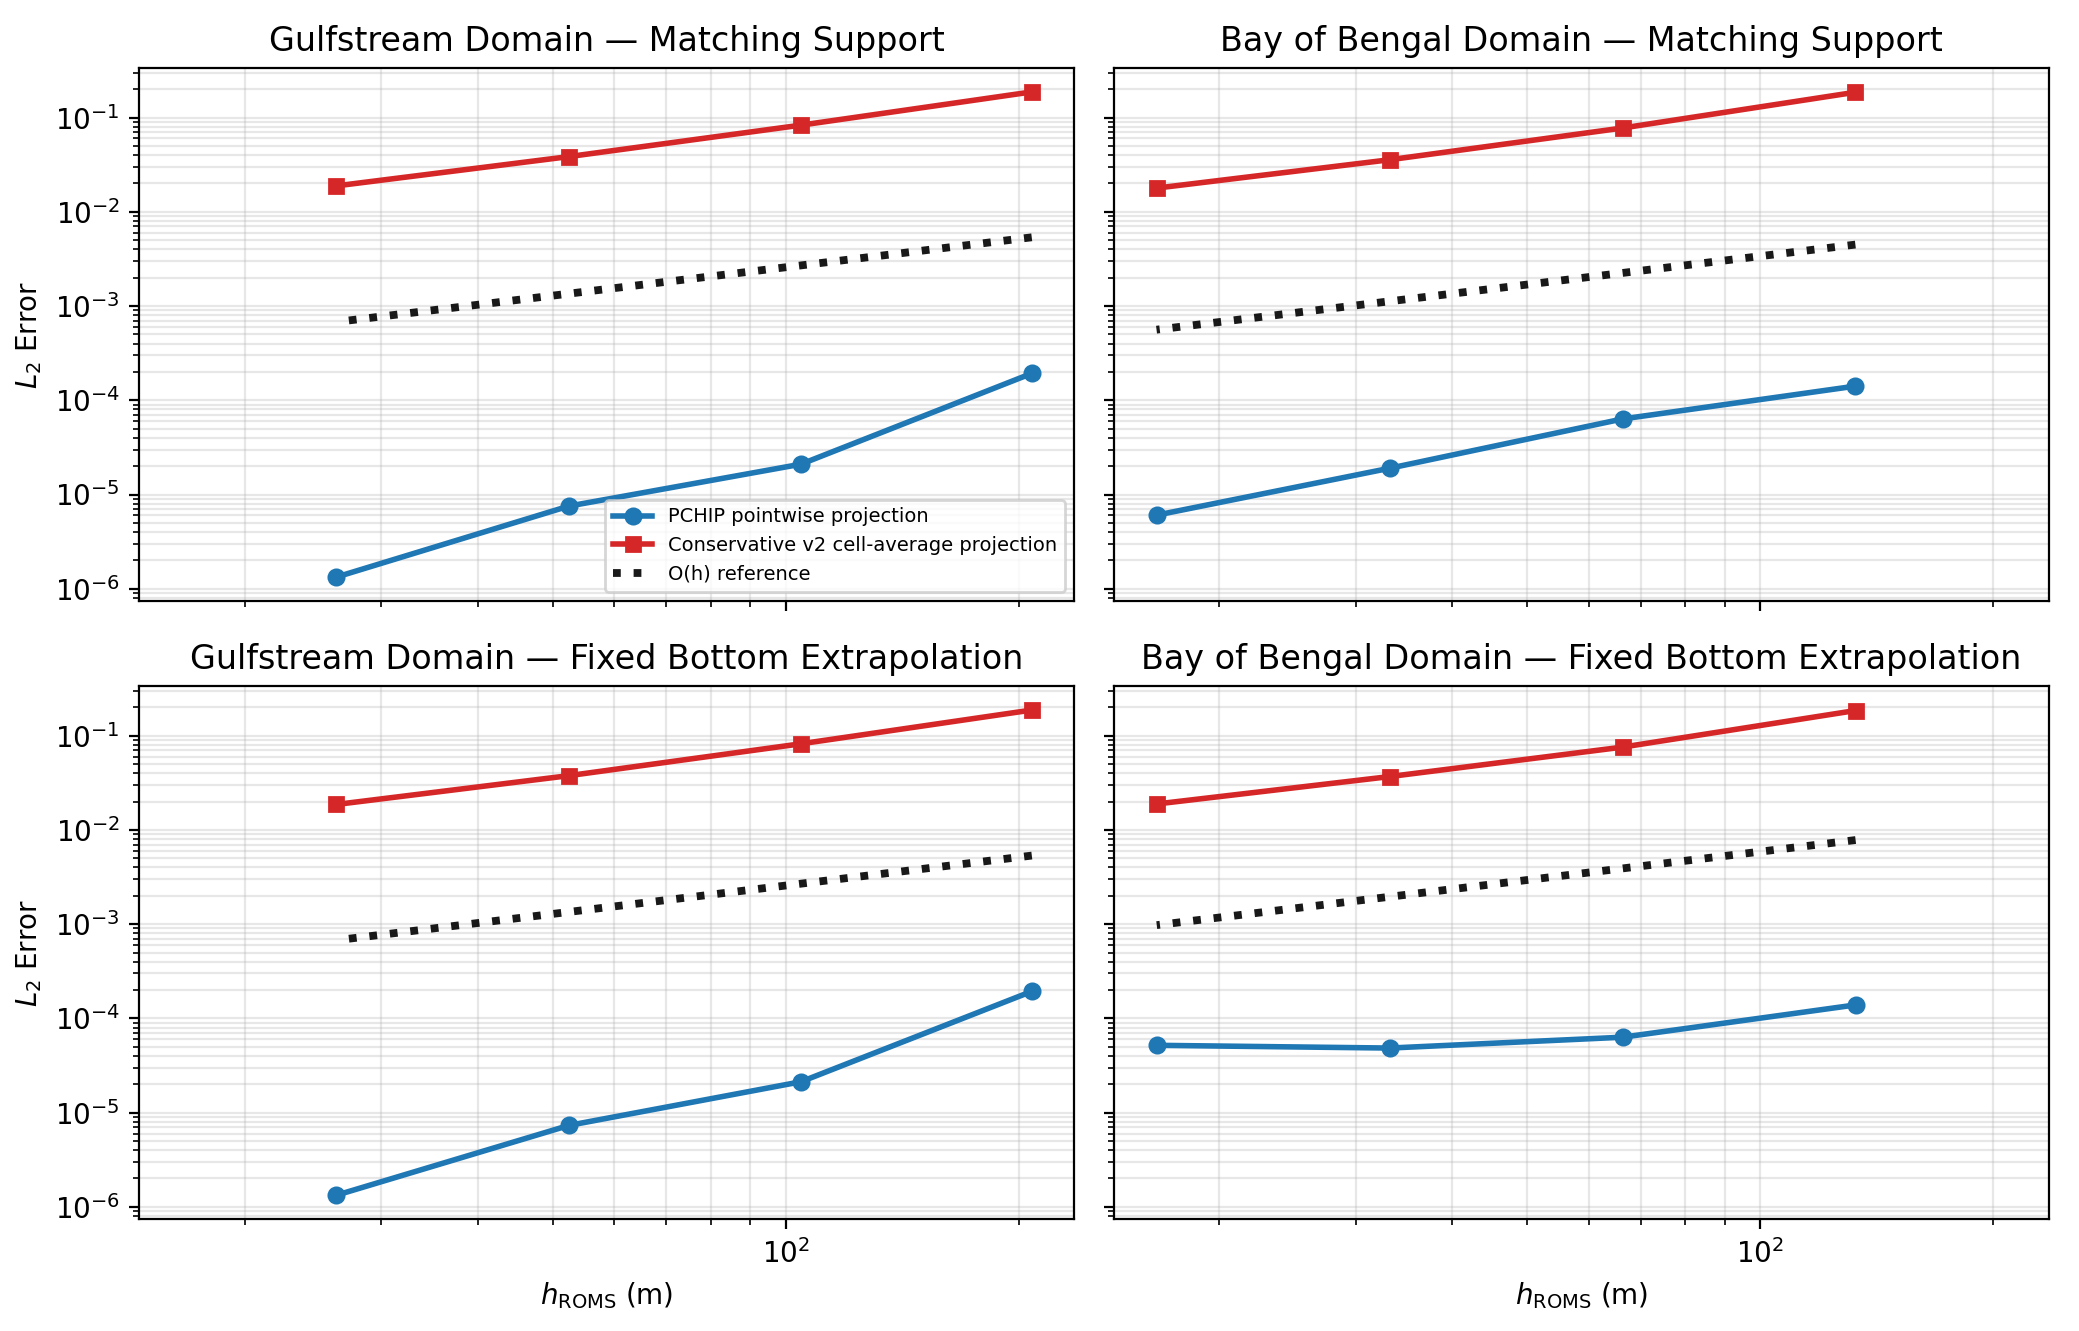
\includegraphics[width=\textwidth]{Figures/conv_1d_convergence.png}
\caption{One-dimensional convergence of the two axial operators. Dotted line: $\mathcal{O}(h)$ reference.}
\label{conv:fig:physical-1d-workflow}
\end{figure}

For the separable transfer in Eq.~\eqref{conv:eq:tensor}, the combined error may be written schematically as
\begin{equation}
  E_{3D}\lesssim C_h h_h^{p_h}+C_z h_z^{p_z}.
  \label{conv:eq:tensor-order}
\end{equation}
When horizontal and axial resolutions are jointly refined at comparable rates, the lower directional observed order in Eq.~\eqref{conv:eq:tensor-order} limits the asymptotic rate of the tensor-product workflow. Thus the observed axial first-order behavior supplies the relevant $\mathcal{O}(h)$ reference for the tested joint refinement. The one-dimensional experiment measures the axial factor only, and it does not independently establish a complete three-dimensional rate or a universal order for every field, mesh, or limiter state.

\subsubsection{Convergence and quantification of error sources}\label{conv:sec:conv}

A convergence study in the usual sense would refine both the \MPAS and \ROMS meshes together. Here the \MPAS global mesh is fixed, as it would be in practice, and we refine only the embedded \ROMS meshes. The sequences below therefore measure how the transfer responds to \ROMS refinement against a fixed \MPAS mesh, not the asymptotic order of the operator.

Figures~\ref{conv:fig:gs-convergence} and~\ref{conv:fig:bob-convergence} show the interior round-trip norms of Eq.~\eqref{conv:eq:norms} versus $\hRatio$ for the two regions. Each panel set reports the volume-weighted $\Lone$ and $\Ltwo$ and the unweighted $\Linf$ for salinity, temperature, the two velocity components, and the smooth analytic field, with scalar errors normalized by representative absolute field magnitudes. Recall from Table~\ref{conv:tab:grid-inventory} that $\hRatio=1$ corresponds to an \MPAS characteristic length of $\SI{9.5}{\kilo\metre}$ in the Gulf Stream and $\SI{16.4}{\kilo\metre}$ in the Bay of Bengal.

%% Gulfstream convergence
\begin{figure}[htbp]
\centering
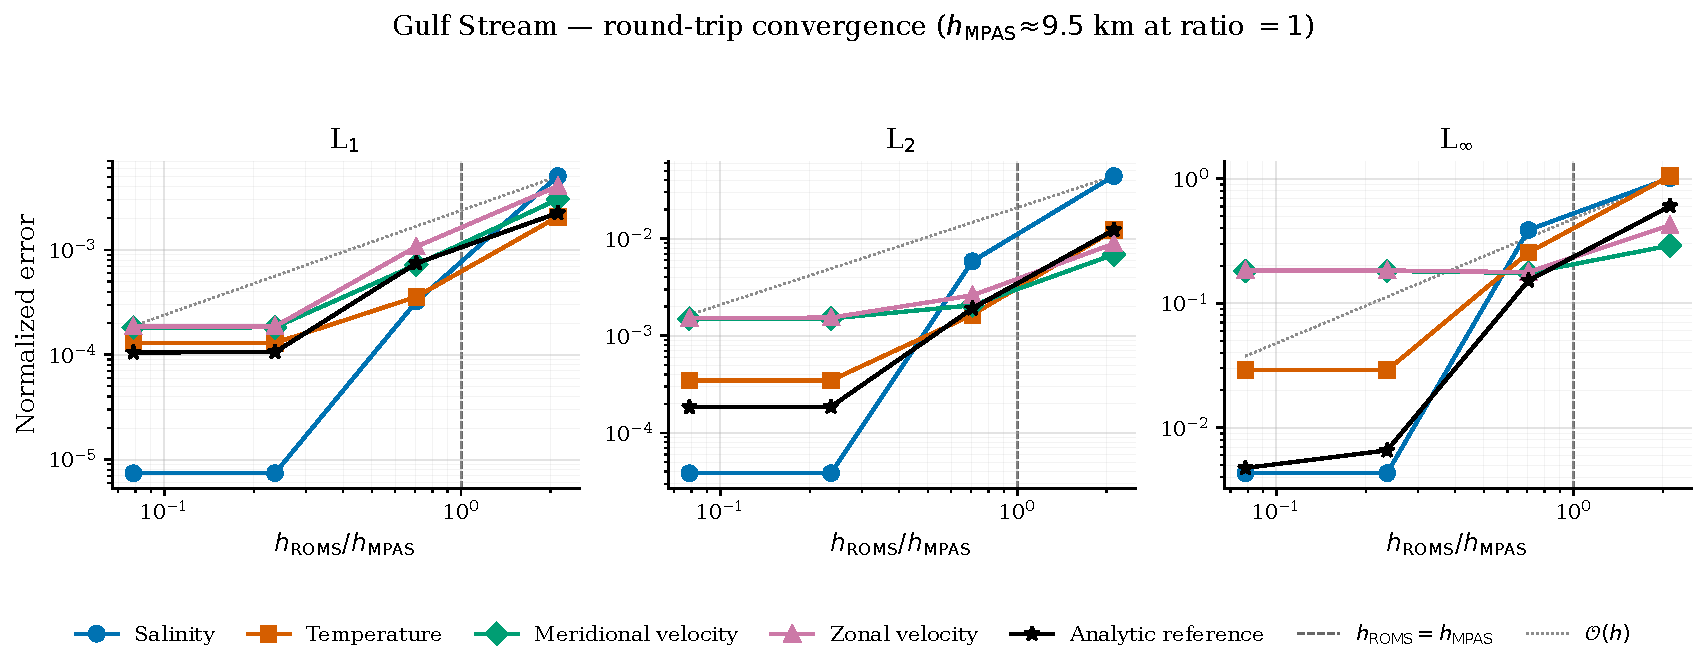
\includegraphics[width=\textwidth]{Figures/conv_convergence_gulfstream.pdf}
\caption{Gulf Stream round-trip errors versus $\hRatio$: $\Lone$ (left), $\Ltwo$ (middle), $\Linf$ (right).}
\label{conv:fig:gs-convergence}
\end{figure}

%% BoB convergence
\begin{figure}[htbp]
\centering
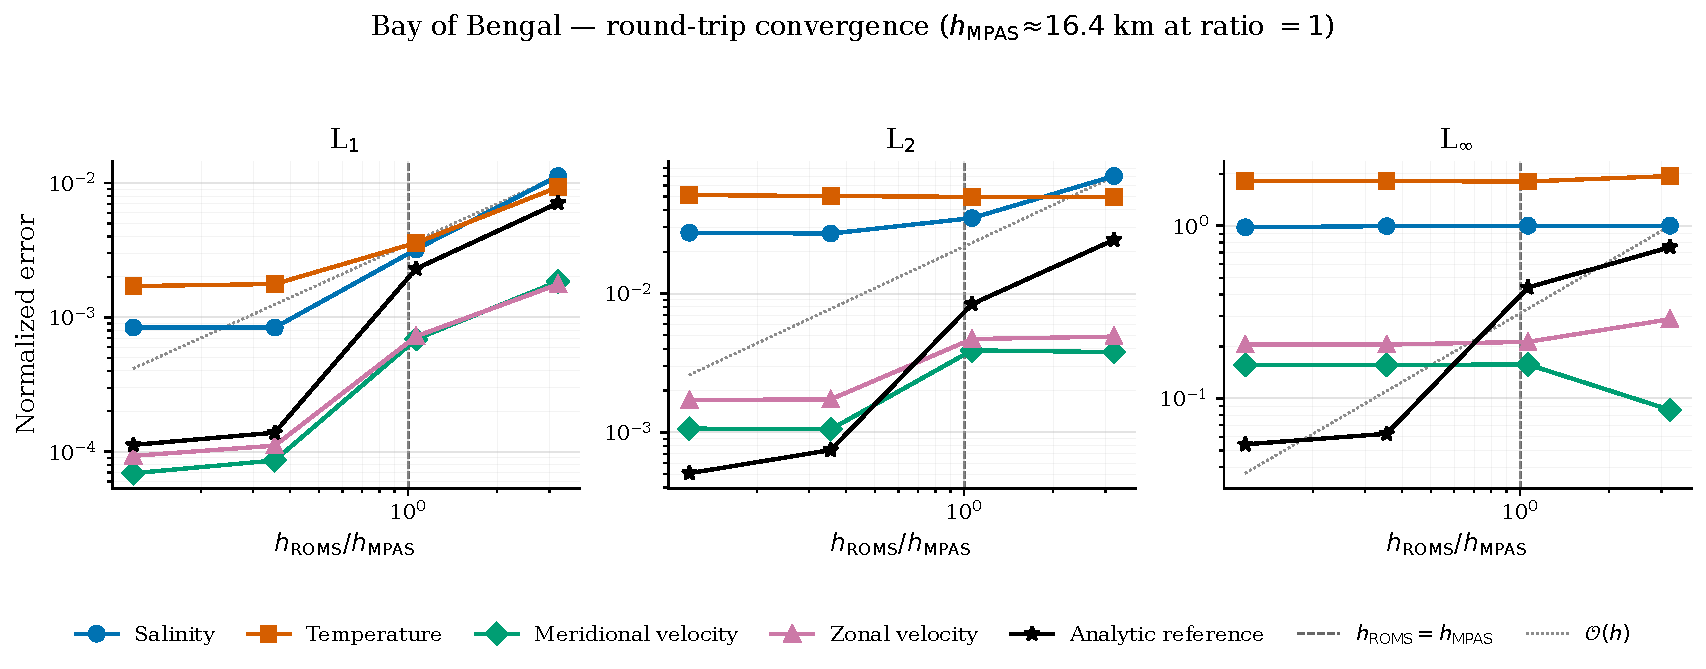
\includegraphics[width=\textwidth]{Figures/conv_convergence_bob.pdf}
\caption{Bay of Bengal round-trip errors versus $\hRatio$: $\Lone$ (left), $\Ltwo$ (middle), $\Linf$ (right).}
\label{conv:fig:bob-convergence}
\end{figure}
\FloatBarrier

Errors decrease over the coarse portion of both sequences, but the real-field errors do not show consistent changes beyond r3 i.e., error plateaus.
%
%The Bay of Bengal r3--r4 comparison deserves particular caution before that plateau is read as a property of the transfer. The number of target columns discarded for lack of a valid vertical reconstruction rises from 18,309 to 166,770 between the two grids, which is 23.0\% and 23.1\% of the respective target cell counts. The discarded region therefore occupies a nearly constant share of the domain, so refinement is not progressively excluding more of it, but that region is resolved differently on the two grids and the norms are evaluated on correspondingly different supports even though the real-field $\Lone$ and $\Ltwo$ values differ by only a few percent. The Gulf Stream sequence discards no columns on any grid, which is consistent with its lack of a land mask and its uniformly deep bathymetry, and it is one reason the two regions should not be compared directly on these norms. A common-support comparison on the finest Bay of Bengal pair would settle whether the plateau is genuine, and we have not run one.
%
Subject to that caveat, the error convergence sequences suggest that $\hRatio\approx0.2$, roughly a fivefold refinement of the \ROMS mesh, is a useful starting point when choosing the \ROMS mesh, and targets at or below $\hRatio\approx0.1$ should be justified by a refinement study for domain of interest when balancing accuracy and computational efficiency. The same value emerges in both an open-ocean and a coastal domain, which is why we offer it as a starting point, but it rests on two domains sharing one \MPAS mesh and a single daily-mean state, so we would recommend confirming it with a short refinement sequence in each new domain rather than adopting it outright.

More generally, for a fixed global \MPAS mesh, a short convergence sequence like this is practical to identify the characteristic length beyond which further refinement of the \ROMS mesh ceases to be worthwhile. As in any multiscale configuration, the lateral boundary conditions supplied from \MPAS carry coarse scale errors that cannot be resolved by \ROMS, or by the forcing itself, as these do not diminish as the \ROMS mesh is refined, so that relative to $\hRatio$ the errors remain $\mathcal{O}(1)$. Because that floor is set by the \MPAS state rather than by the transfer, refining past the point where the sequence flattens buys little in the fidelity of the transferred fields, though we have not measured what it does to the regional solution that evolves from them. The cost, meanwhile, continues to grow: the number of \ROMS cells scales as $\hRatio^{-2}$ and a CFL-limited time step shrinks in proportion to the characteristic length, so integrating a fixed period becomes roughly $\hRatio^{-3}$ more expensive. Choosing the \ROMS characteristic length near the flattening point therefore captures most of the accuracy that the \MPAS state makes available, at a small fraction of the cost of the finest grids tested here. We did not run targets below $\hRatio\approx0.08$, so this is an argument about the range examined rather than an asymptotic claim.

The convergence order of the composed scheme is determined by the rate of the horizontal and vertical components. Imposing conservation on the vertical operator such that each \ROMS layer integral in the reconstructed profile matches the contributions from the \MPAS geopotential coordinate topology, the vertical projection operator mimics a traditional $L_2$ minimization in one dimension, resulting in a first order approximation in the layer thickness. Since the tensor product in Eq.~\eqref{conv:eq:tensor} is no more accurate than its least accurate factor, the composed three-dimensional transfer is first order overall, irrespective of the formal accuracy of the horizontal map. The measured decrease over the convergent portion of both sequences is consistent with this expectation, although four grids are too few to fit an asymptotic rate.

Relaxing the conservation constraint admits alternatives, and this choice is an application decision rather than a purely numerical one. A quasi-interpolant that reproduces the profile rather than its layer integrals reaches higher order on smooth fields, as the one-dimensional comparison of \S\ref{conv:sec:axial-refinement} shows, but forfeits exact conservation, monotonicity, or both depending on how it is constructed. Higher order bought by violating monotonicity can introduce spurious extrema in sharp features such as the thermocline, and a scheme that sacrifices conservation is poorly suited to long integrations where tracer inventories must be maintained. For boundary and initial-condition forcing of a regional model that carries its own conservative transport, either trade may be defensible, and we chose conservation.
%
%\subsubsection{Separating target refinement from the parent representation}\label{conv:sec:controlled}
%
%Because the round trip chains the forward and reverse horizontal maps with the forward and reverse vertical remaps, it cannot by itself indicate which stage limits the result. We did not decompose the operator into horizontal-only and vertical-only legs, which is what would attribute the floor to a specific stage. What the controlled experiments below do instead is hold the \MPAS source fixed while refining only the \ROMS target, which separates the effect of target spacing from the effect of the parent representation without isolating either map. A constant field carried forward and back through the horizontal map alone is reproduced to roundoff, as required by the normalization in Eq.~\eqref{conv:eq:bilin-weight}. In the tensor product split, the composed one-way error, measured against the analytic solution sampled on the target grid, then varies by about 4\% in the Gulf Stream and 5\% in the Bay of Bengal across the whole r1--r4 sequence, which is what we expect when the fixed parent representation, rather than the target spacing, sets the achievable accuracy. The round trip over the same sequence falls by roughly a factor of 23 and 30 respectively, since errors incurred on the forward leg can be undone on the reverse leg, so the round trip is not the one-way error plus a correction, and the two should not be compared directly. These statements apply to the controlled analytic configuration and do not settle the real-field r3--r4 common-support caveat.
%
%Errors grow with depth, and the salinity floors in the two regions differ by about two orders of magnitude. We cannot attribute that gap: the two regions differ in source resolution, in coastal gradient strength, and in the extent of their land masks, and the round-trip metric does not separate these. The persistent $L_\infty$ salinity errors are localized near the surface and near coastlines, and their location shifts with refinement, which is consistent with under-resolved near-surface stratification but does not establish it.


%\FloatBarrier
%\subsection{Performance}\label{conv:sec:performance}
%The benchmark projects four fields from a source mesh of $5.7\times10^6$ polyhedra to a target mesh of $8\times10^6$ elements on one Perlmutter CPU node, using 1--64 OpenMP threads and $N_z=50$ and 100.
%
%\begin{figure}[htbp]
%\centering
%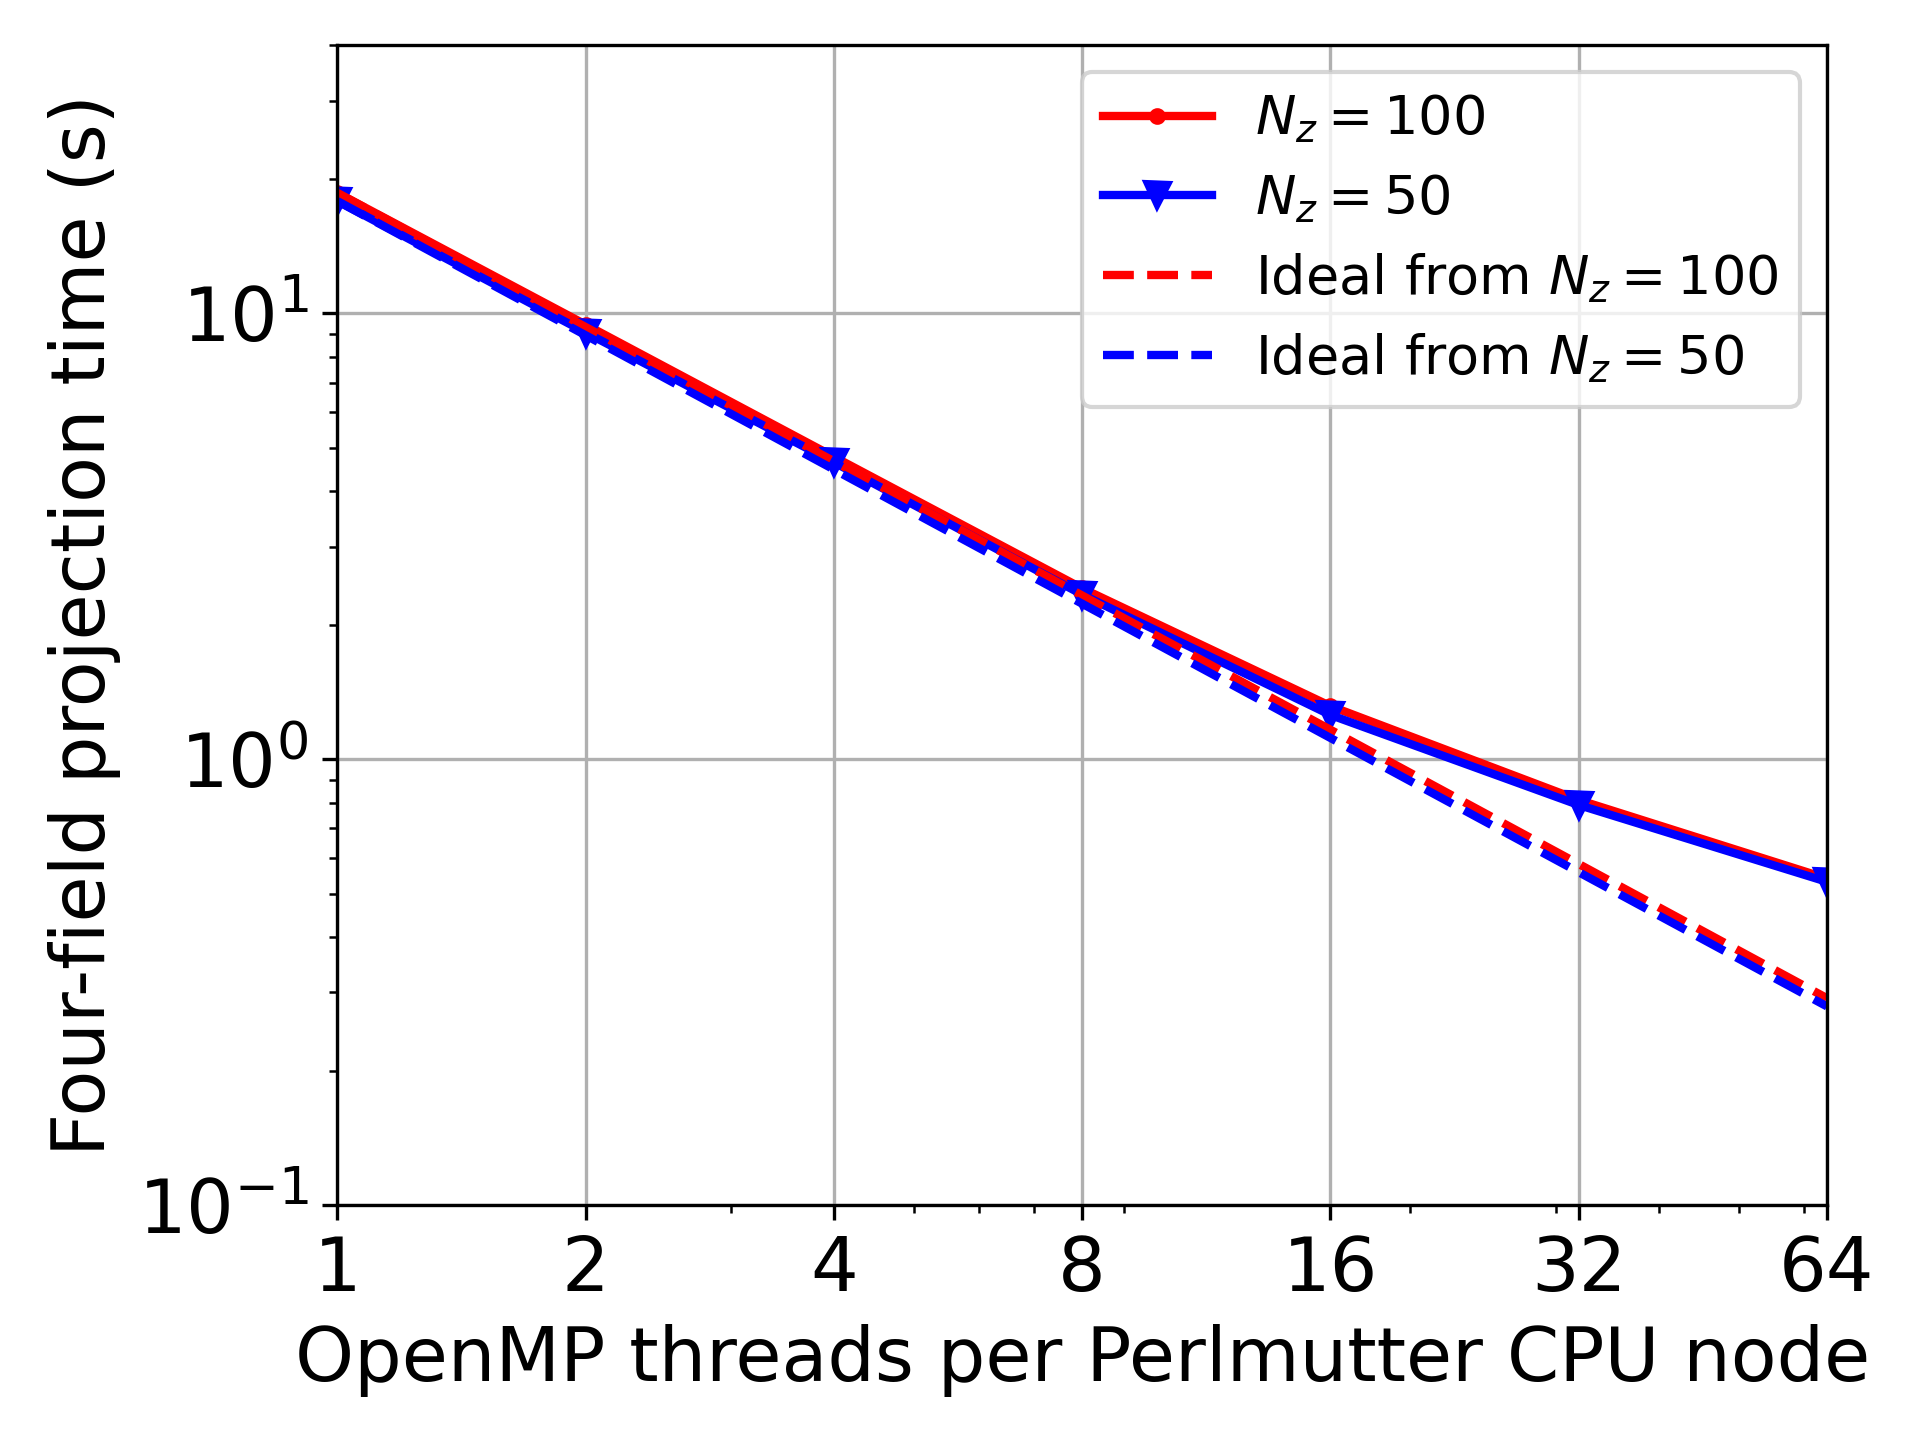
\includegraphics[width=0.7\textwidth]{Figures/conv_omp_scaling_perlmutter.png}
%\caption{Strong scaling of the four-field projection at $N_z=50$ and $N_z=100$.}
%\label{conv:fig:omp-scaling}
%\end{figure}
%\FloatBarrier
%
%Figure~\ref{conv:fig:omp-scaling} shows a measured speedup of $34.5\times$ at $N_z=100$ and $33.6\times$ at $N_z=50$, corresponding to an average of 53\% strong-scaling parallel efficiency at 64 threads, while the two vertical-resolution curves nearly overlap. The resuls for the run are averaged over 10 executions, and showcase the net volumetric remapping speedup rather than separately quantifying the cost of the horizontal and vertical phases of the remap.

\subsection{Bathymetry treatment and regional applications}\label{conv:sec:bathysmooth}
The projected bathymetry can generate sigma-coordinate pressure-gradient errors over steep slopes~\citep{haney1991pressure,mellor1994pressure}. We condition it with a one-ring log-depth averaging smoother. Writing $H_i$ for the depth of \ROMS cell $i$, $q_i=\log H_i$ for its logarithm, $\mathcal{A}(i)$ for the set of edge-neighbours of that cell, and $m$ for the iteration counter, each sweep replaces the log-depth of a cell by the mean over its one-ring neighbourhood,
\begin{equation}
 q_i^{(m+1)}=\frac{1}{|\mathcal{A}(i)|}\sum_{i'\in\mathcal{A}(i)}q_{i'}^{(m)},\qquad H_i^{(m+1)}=\exp q_i^{(m+1)},
 \label{conv:eq:onering}
\end{equation}
with clipping to the \MPAS range. Operating on $\log H$ rather than $H$ makes the smoother act on relative rather than absolute depth differences, so a given number of sweeps has comparable effect on the shelf and in the deep ocean. Land cells are excluded from the neighbourhood sums. Smoothing by Eq.~\eqref{conv:eq:onering} stops once the steepest remaining neighbour contrast satisfies
\begin{equation}
 r_{\max}^{(m)}=\max_i\max_{i'\in\mathcal{A}(i)}\frac{q_i^{(m)}-q_{i'}^{(m)}}{q_i^{(m)}+q_{i'}^{(m)}}<0.05,
 \label{conv:eq:slope-stop}
\end{equation}
which is the sole termination condition, with no cap on the iteration count. Evaluated on the same log-depths, this test plays the role of the $r$-factor conventionally used to condition terrain-following grids~\citep{sikiric2009smoothing}. The resulting bathymetry is shown in Fig.~\ref{conv:fig:smoothing}.

\begin{figure}[htbp]
\centering
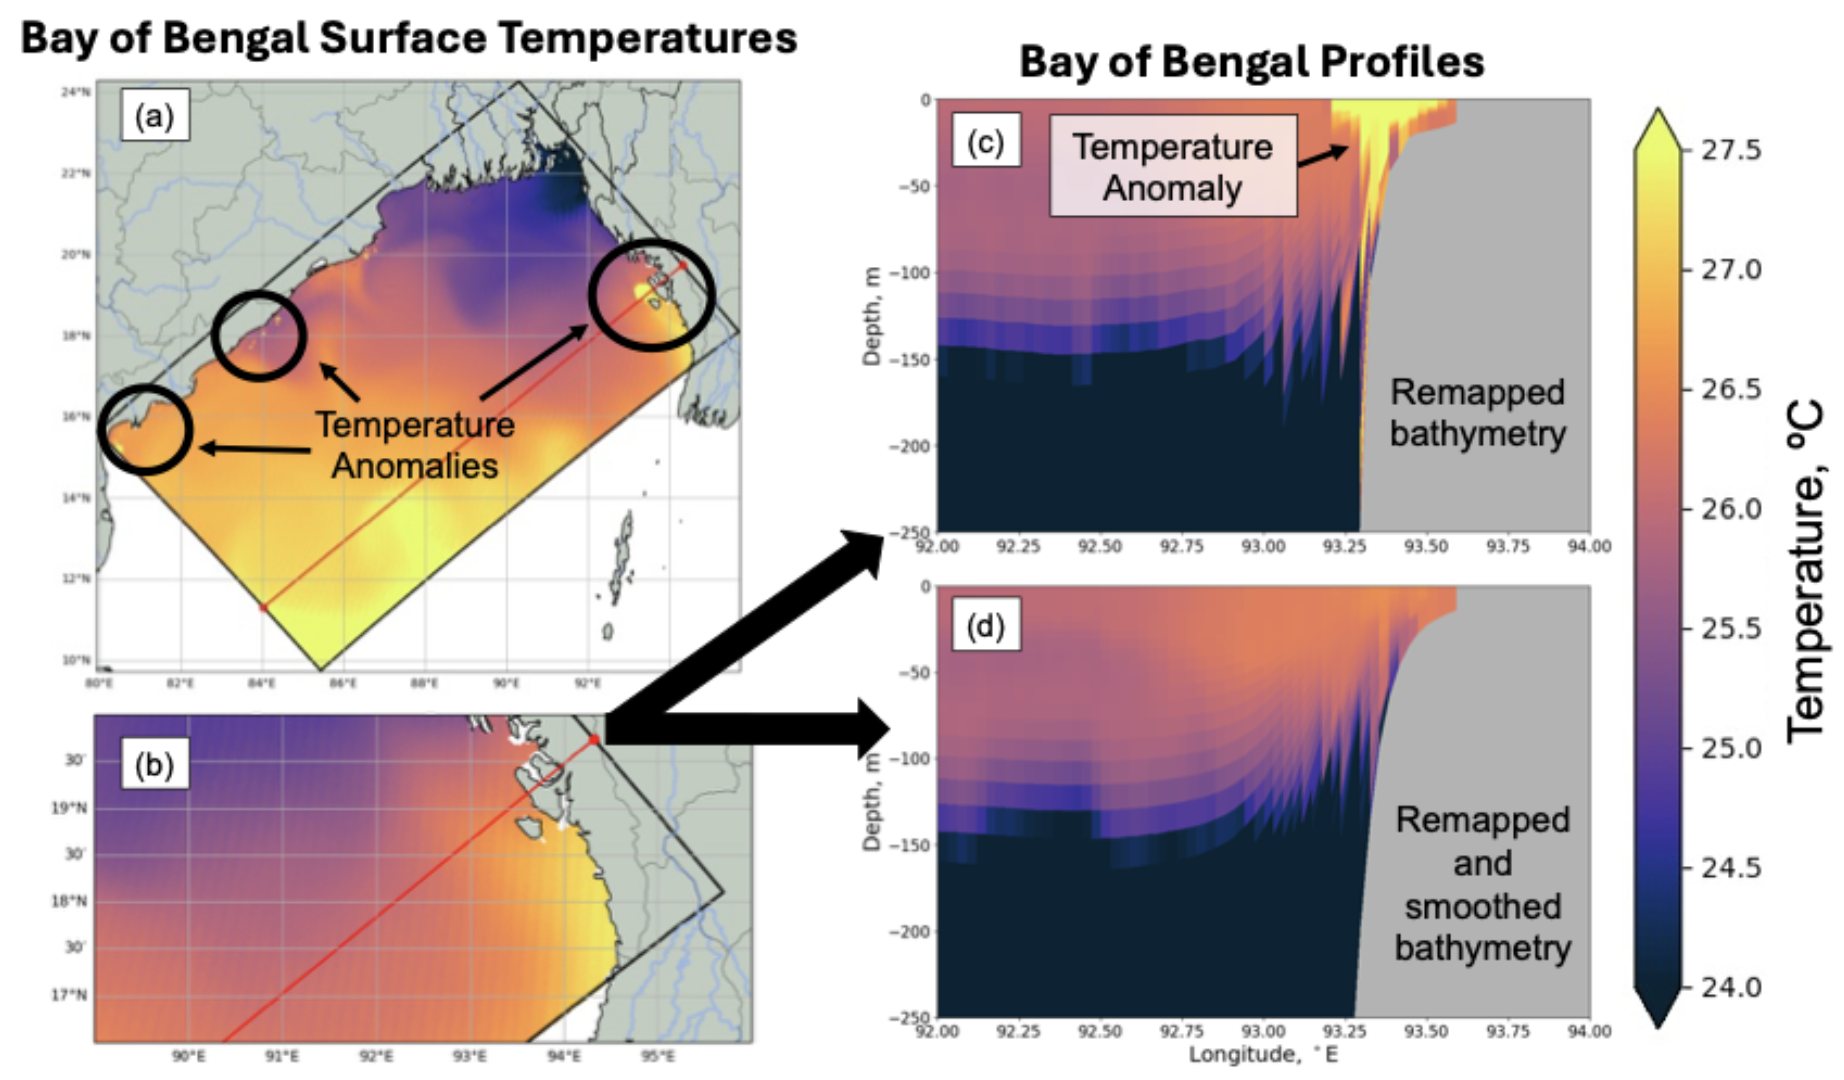
\includegraphics[width=\textwidth]{Figures/conv_bathy_smoothing.png}
\caption{Projected Bay of Bengal bathymetry before and after smoothing.}
\label{conv:fig:smoothing}
\end{figure}
\FloatBarrier

Smoothing the logarithm of the bathymetry changes the round-trip errors by less than 5\% and was sufficient to stabilize the Bay of Bengal integration. That domain also required vertical smoothing of the remapped scalar profiles, which removed a warm anomaly between 100 and 200 m near masked coastlines. The two treatments act on different quantities and we report their effects separately. Elsewhere the regional applications use the projected \MPAS geometry, except where coastal or estuarine topography forces us to blend it with the native \ROMS bathymetry and to retain the \ROMS land mask. Chesapeake Bay is the clearest example: the \MPAS mesh cannot represent the estuarine geometry at all, so the boundary and initial fields there must be prescribed or blended, and the blending weights we used are not specified precisely enough for the case to be reproduced.


Running \ROMS on finer regional meshes with \MPAS-derived boundary conditions produces finer-scale spatial variability across the regional domains (Fig.~\ref{fig:zeta_snapshots}). The kinetic-energy records change relative to the parent and directly remapped states in a domain-dependent way (Fig.~\ref{fig:region_KE}), reflecting both the transferred state and the variability generated by the regional dynamics. Chesapeake Bay is shown separately in Fig.~\ref{fig:chesResults} because its estuarine geometry requires blending. \REVIEWc{Kyle} The figures in this subsection illustrate what the downscaled simulations produce and they clearly show that submesoscale processes are born, evolve and propagate under regional refinements, which are averaged over by the global coarse scale models. \TODOc{add more}

\begin{figure}[htbp]
\centering
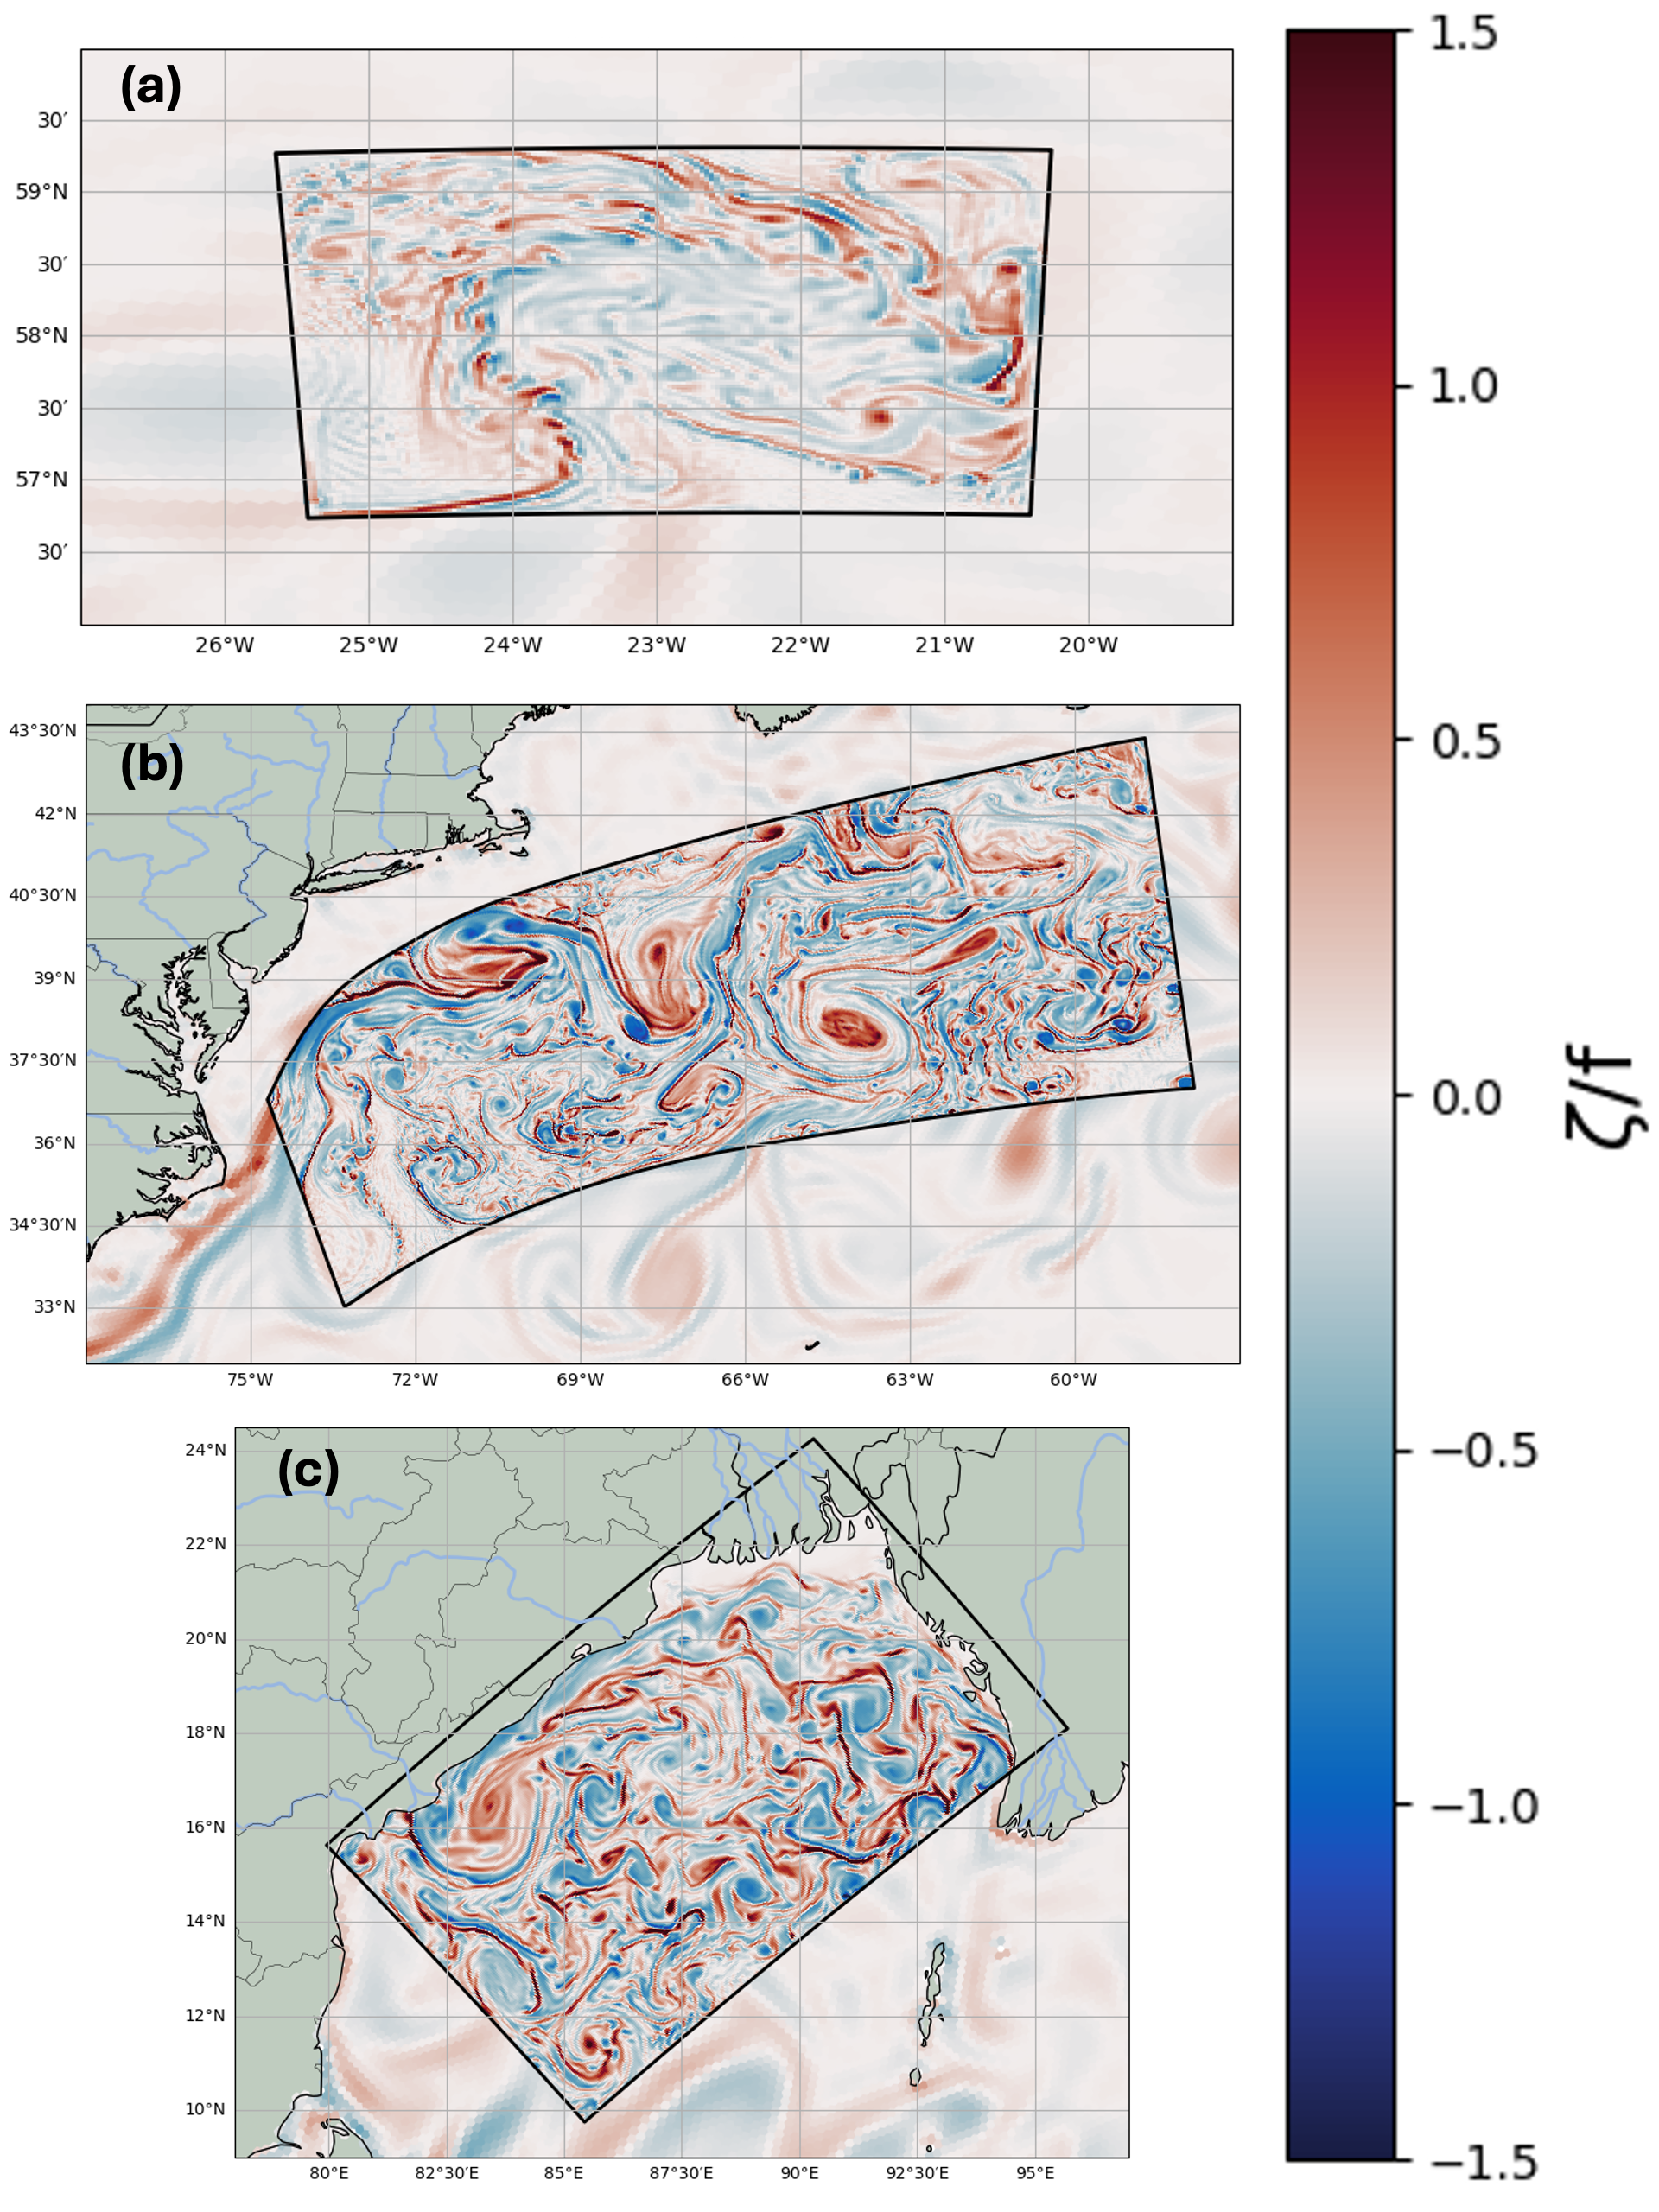
\includegraphics[width=0.90\textwidth]{Figures/zeta_3domains_v0.png}
\caption{Surface relative-vorticity fields for the North Atlantic, Gulf Stream, and Bay of Bengal regional domains.}
\label{fig:zeta_snapshots}
\end{figure}

\TODOc{Introduce and talk about benchmarks for regional domains and how these are validated}


\begin{figure}[htbp]
	\centering
	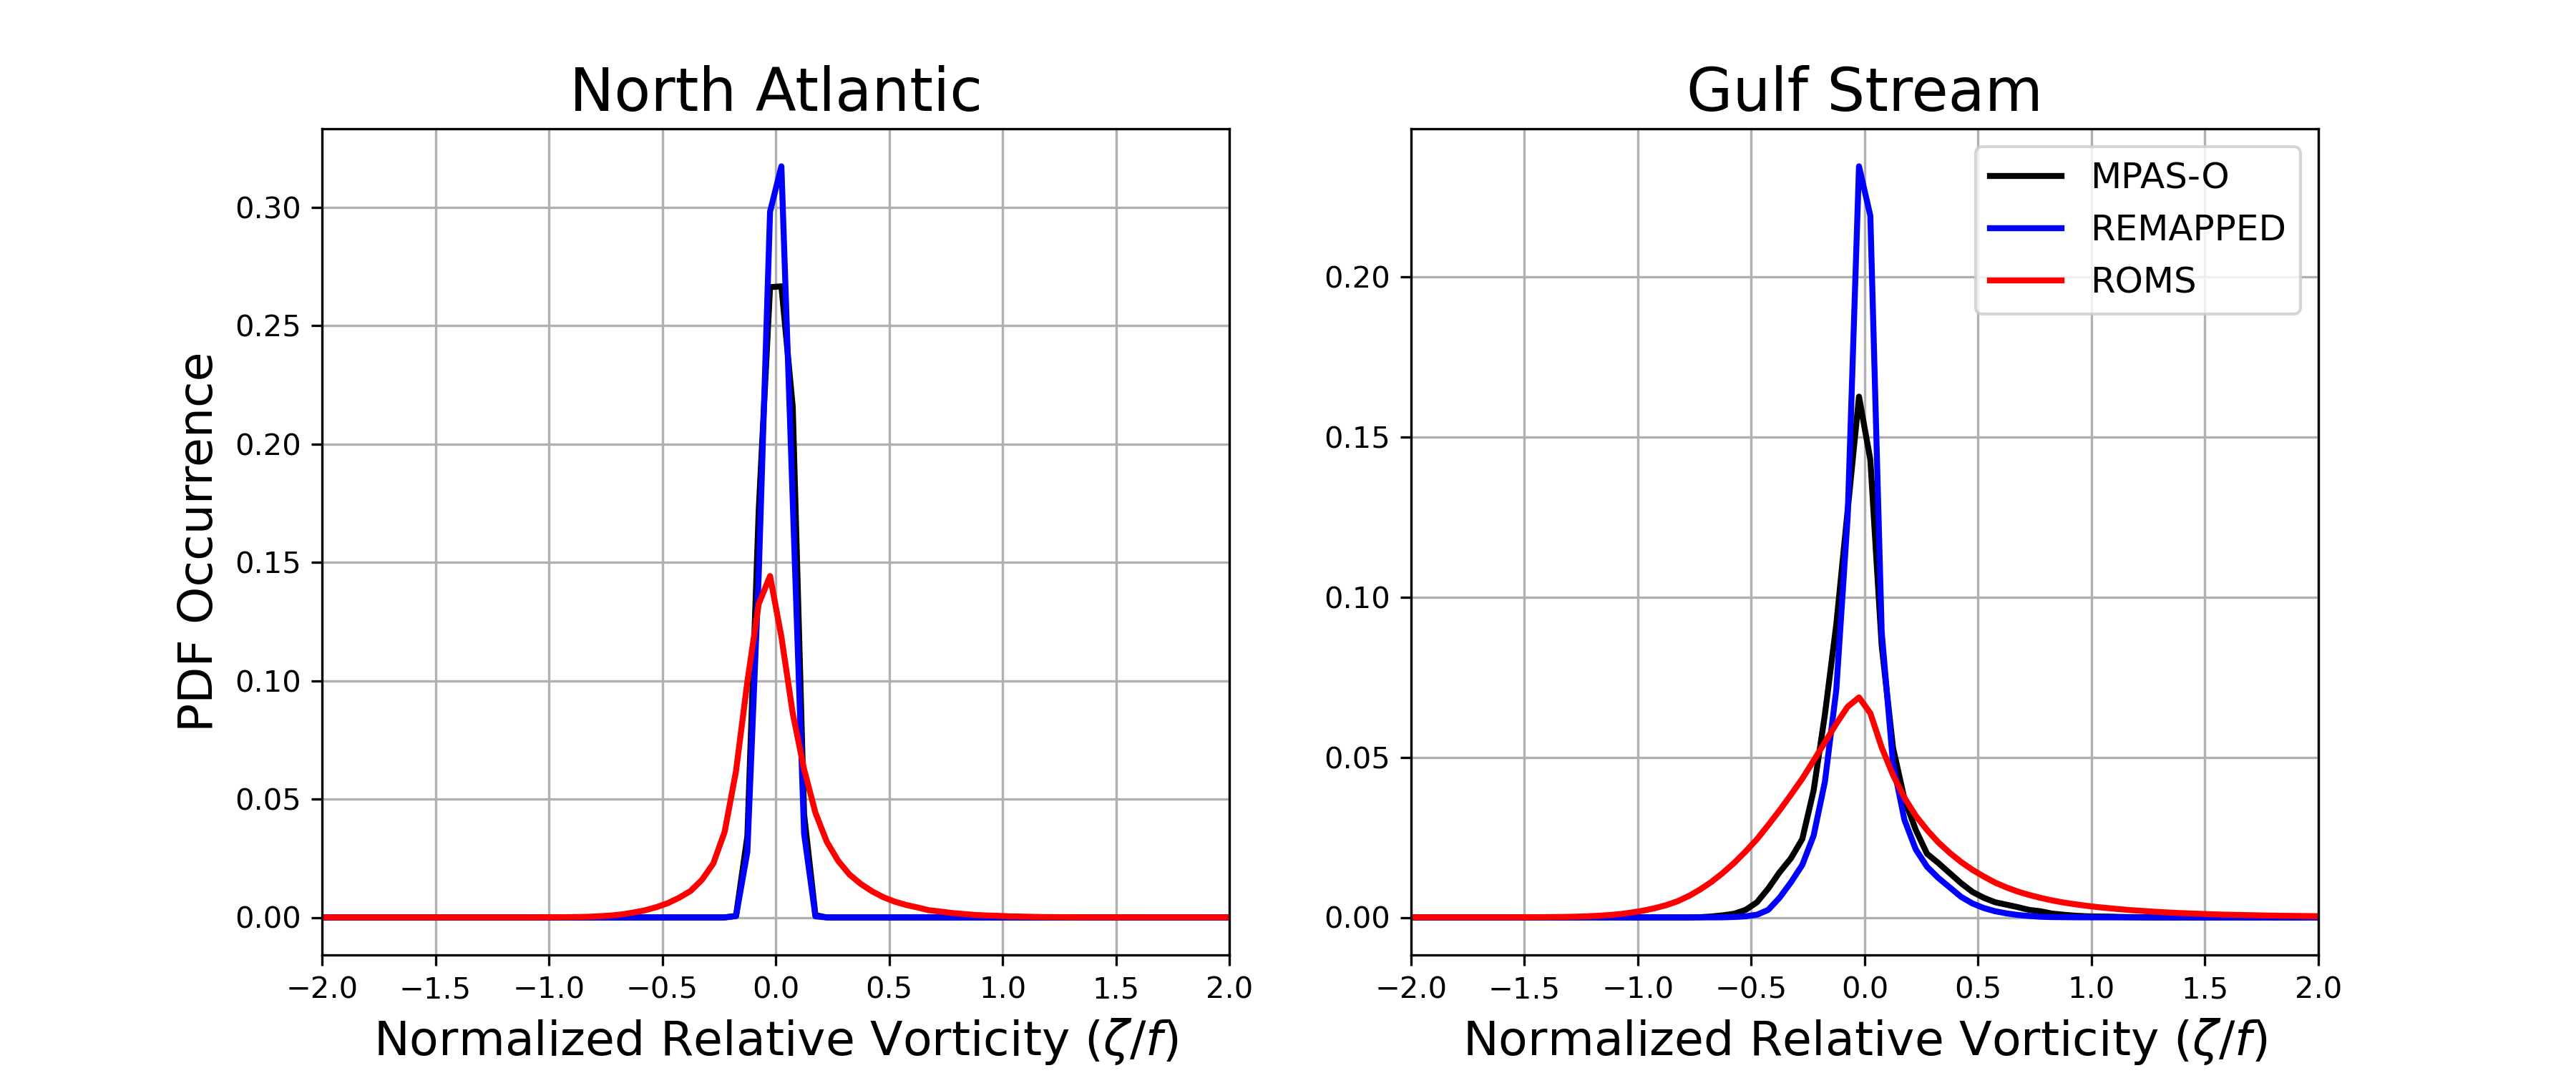
\includegraphics[width=0.88\textwidth]{Figures/regional_zeta.png}
	\caption{Normalized relative vorticity distribution for Niskine and Gulfstream cases.}
	\label{fig:relVortPDF}
\end{figure}
\FloatBarrier


The surface kinetic energy used in Fig.~\ref{fig:region_KE} is defined by
\begin{equation}
  \mathrm{KE}=\frac{1}{2}\left(u^2+v^2\right)\quad [\si{\metre\squared\per\second\squared}],
  \label{conv:eq:ke}
\end{equation}
with velocities represented at cell centers for the diagnostic.

\begin{figure}[htbp]
\centering
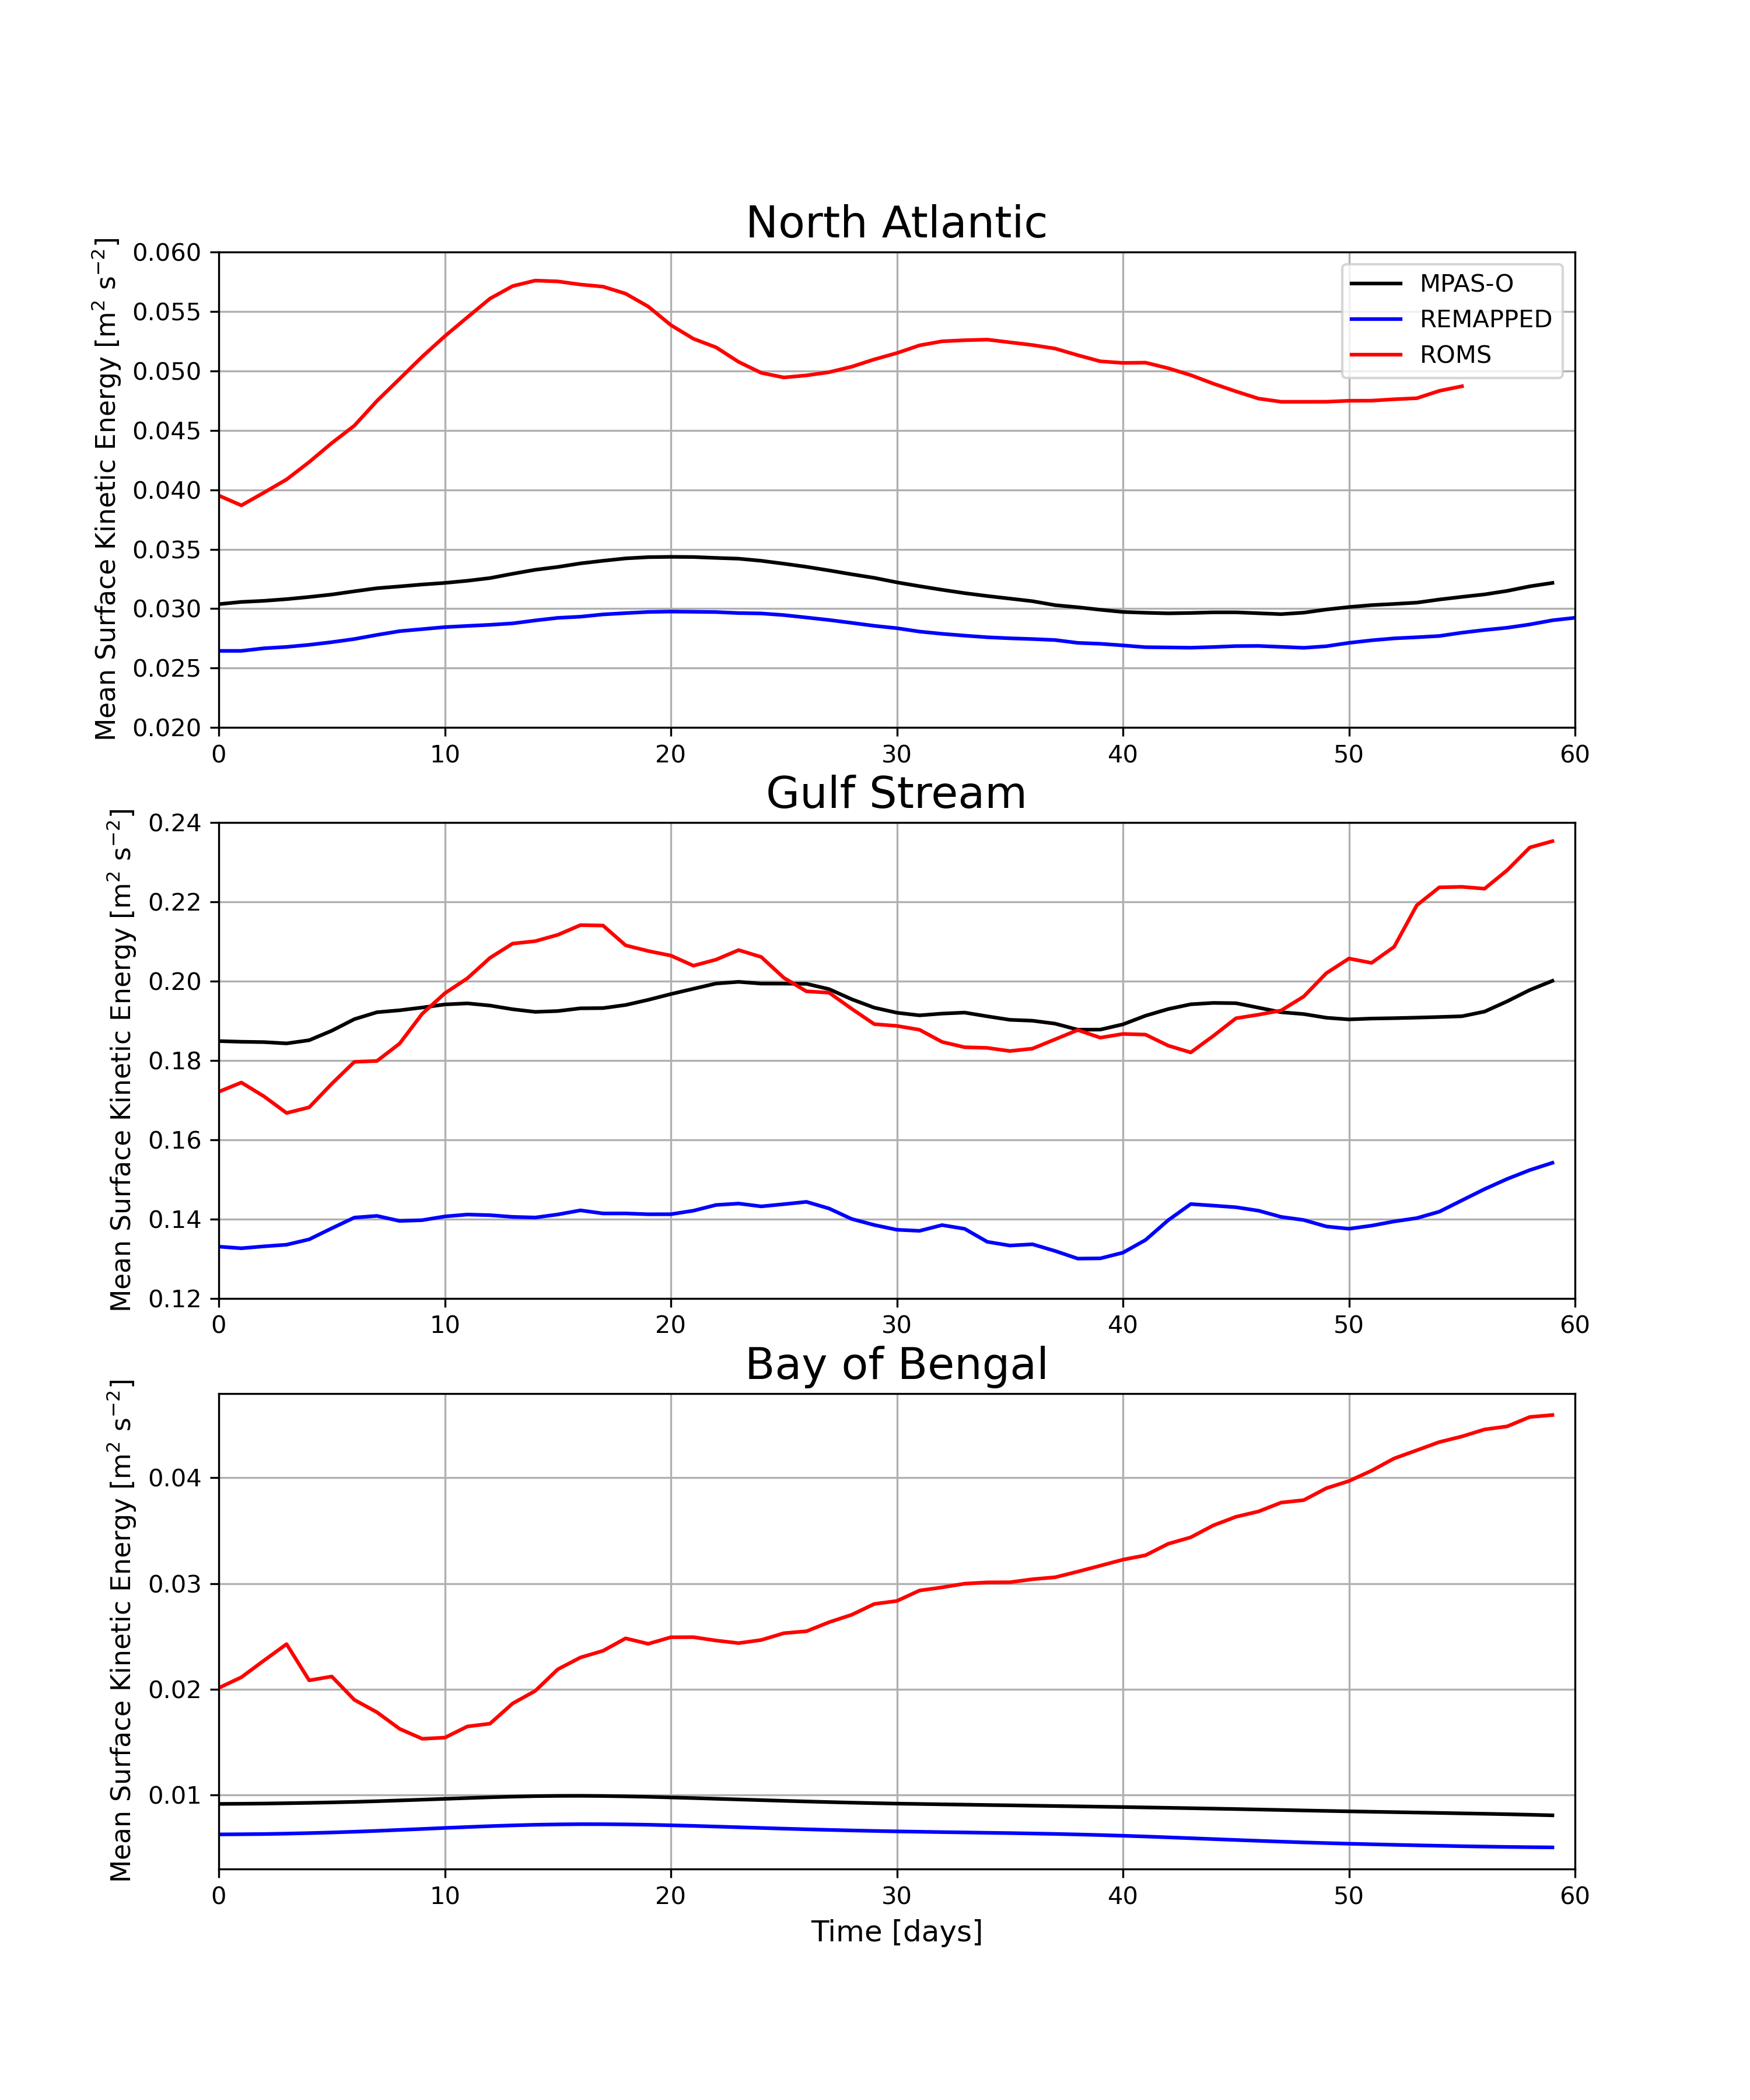
\includegraphics[width=\textwidth]{Figures/Region_KE_TimeSeries_3domains.png}
\caption{Surface specific kinetic-energy time series for the North Atlantic, Gulf Stream, and Bay of Bengal domains, evaluated with the diagnostic definition in Eq.~\eqref{conv:eq:ke}.}
\label{fig:region_KE}
\end{figure}

\begin{figure}[htbp]
\centering
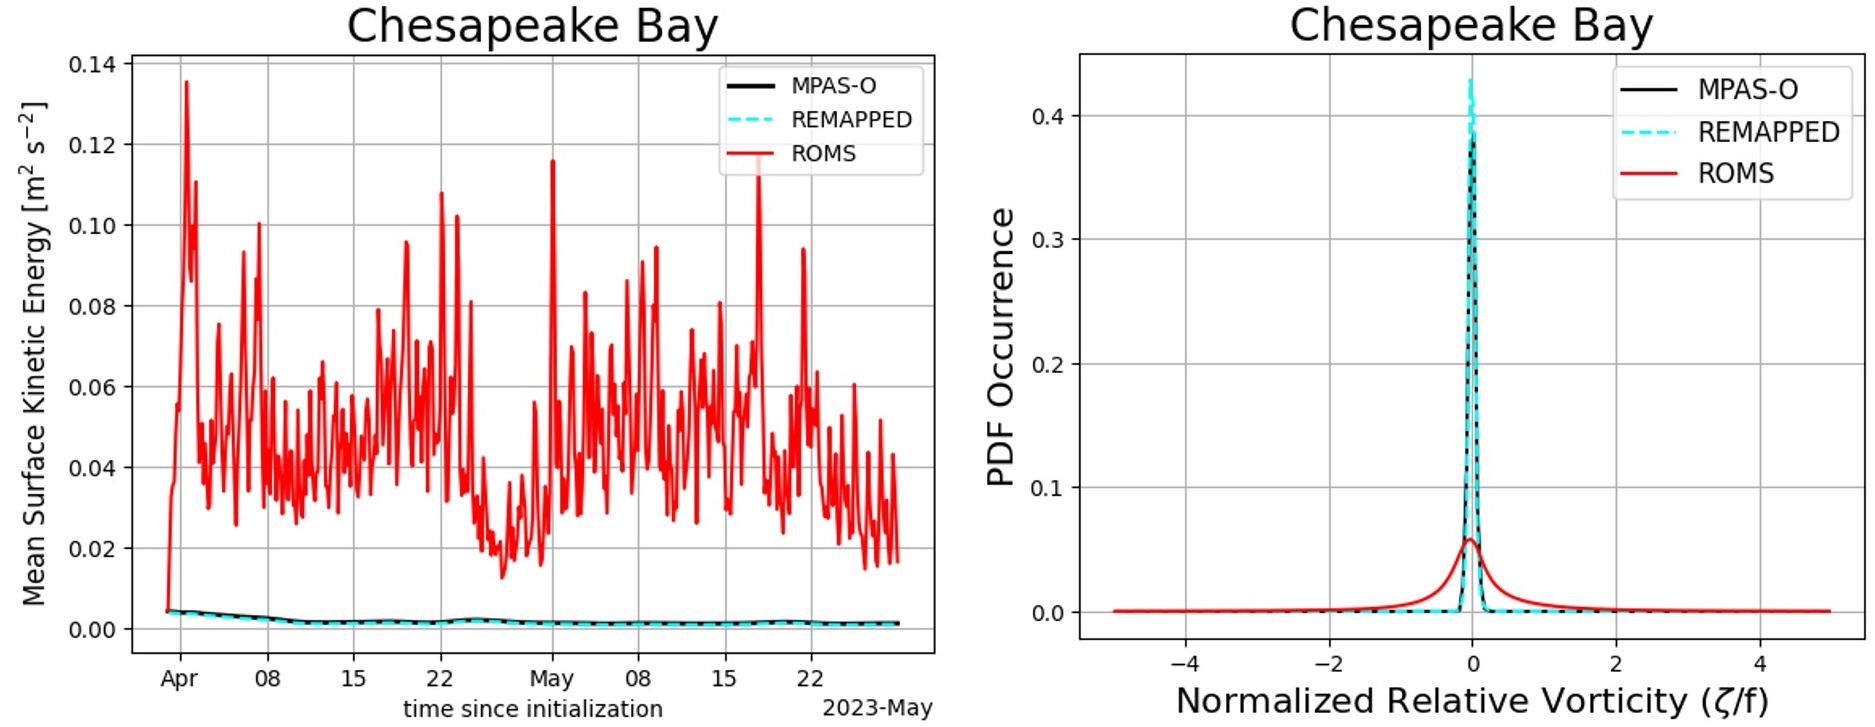
\includegraphics[width=0.88\textwidth]{Figures/chesbay_ke_zeta.jpg}
\caption{Surface specific kinetic energy and relative-vorticity distribution for Chesapeake Bay. These estuarine results are preliminary.}
\label{fig:chesResults}
\end{figure}
\FloatBarrier

The open-ocean and coastal applications occupy relative target scales near $\hRatio\approx0.2$--$0.35$, whereas Chesapeake Bay is substantially finer relative to its parent. In every domain the regional solution alters both the geometry of the flow and its energy content relative to the parent state. Because the regional model continues to evolve after initialization, these differences measure the combined effect of the transfer and the subsequent regional dynamics, and the convergence experiments of Sect.~\ref{conv:sec:conv} remain the quantitative statement about the transfer itself. The Chesapeake result depends particularly strongly on native bathymetry, land-mask treatment, and the blended estuarine fields. \TODOc{talk more about practical implementation of this case}

